\documentclass[border=0.2cm]{standalone}

\usepackage{tikz}
\usetikzlibrary{shapes.geometric}
\begin{document}

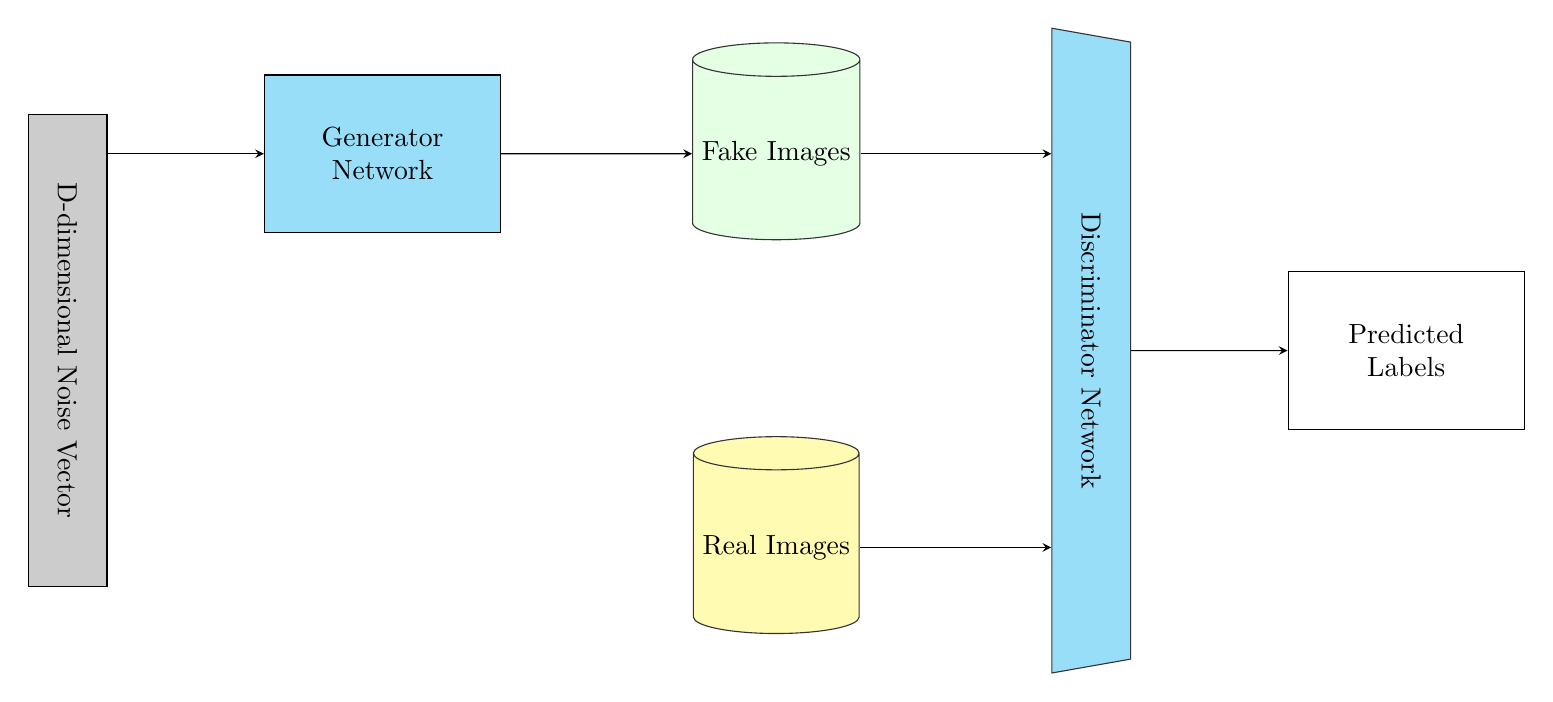
\begin{tikzpicture}

\node[cylinder, draw = black!80, text = black, fill = green!10, minimum height = 2.5cm, aspect = 0.2, shape border rotate = 90] (fakeimg) at (0,2.5) {Fake Images};

\node[cylinder, draw = black!80, text = black, fill = yellow!30, minimum height = 2.5cm, aspect = 0.2, shape border rotate = 90, below of=fakeimg, node distance=5cm] (realimg) {Real Images};

\node (rect) [draw,fill=cyan!40,minimum width=3cm,minimum height=2cm, align=center, left of=fakeimg, node distance=5cm] (gennet)  {Generator \\Network};

\node[trapezium, draw = black!80, text = black, align=center, fill = cyan!40, trapezium angle=80, minimum height=1cm, rotate=270] (t1) at (4,0) { Discriminator Network};  

\node (rect) [draw, minimum width=3cm,minimum height=2cm, align=center, right of=t1, node distance=4cm] (predlabel)  {Predicted \\Labels};

\node (rect) [draw,fill=black!20,minimum width=6cm,minimum height=1cm, rotate=-90] (noisevect) at (-9,0) {D-dimensional Noise Vector};


\draw [-stealth] (t1.north) -- (predlabel.west) node[midway,right] {};
\draw [-stealth] (fakeimg.east) -- (t1.south|-fakeimg.east) node[midway,right] {};
\draw [-stealth] (realimg.east) -- (t1.south|-realimg.east) node[midway,right] {};
\draw [-stealth] (gennet.east) -- (fakeimg.west) node[midway,right] {};
\draw [-stealth] (noisevect.north) --  node[right=3pt] {} ++(0,3) |- (gennet.west) {};

\end{tikzpicture}
 
\end{document}
